\documentclass[notheorems]{beamer}
\usepackage[numbers]{natbib}
\setcitestyle{open={[},close={]}}
\renewcommand{\bibsection}{} %no references section

\usepackage{tcolorbox}
% Slide colors
\usetheme[progressbar=frametitle, progressbar linewidth=1pt]{moloch}
\definecolor{utorange}{RGB}{191, 87, 0}
\definecolor{utblack}{RGB}{51, 63, 72}
\definecolor{uttangerine}{RGB}{248, 151, 31}
\definecolor{cffffff}{RGB}{255,255,255}
\definecolor{utlimestone}{RGB}{214, 210, 196}
\definecolor{utsunshine}{RGB}{255, 214, 0} %UT colors


\definecolor{Main}{HTML}{BF5700} %duplicate of utorange
\definecolor{Accent1}{HTML}{f8971f}
\definecolor{Accent2}{HTML}{005f86} %my color scheme

\setbeamercolor{alerted text}{fg=Accent2} %TK
\setbeamercolor{example text}{fg=utorange}
\setbeamercolor{palette primary}{bg=utorange}
\setbeamercolor{bibliography entry location}{fg=utorange}
\setbeamercolor{frametitle}{bg=utorange, fg=cffffff}
\setbeamercolor{progress bar}{fg=utorange,bg=Accent2}
\setbeamercolor{background canvas}{bg=white}

\setbeamertemplate{frame footer}{\insertshortauthor ~ \hfill\insertshorttitle}

\setbeamerfont{page number in head/foot}{size=\tiny}
\setbeamercolor{footline}{fg=utblack}

\usefonttheme{serif} %fuck sans serif 

% Theorems
\tcbuselibrary{skins}
\tcbuselibrary{breakable}
\tcbuselibrary{theorems}

\newtcbtheorem[number within=subsection,
    %number freestyle={\noexpand\thesection.\noexpand\thesubsection.\noexpand\Roman{\tcbcounter}} %for use with revtex
    number freestyle={\noexpand\arabic{\tcbcounter}} %for tufte
    ]{olddefinition}{\vphantom{Apgjy}Definition}{breakable, 
    parbox=false, %bitch what TK i'm gonna kill myself this fixed the stupid shit TK what is the stupid shit i fucking forgot maybe the tim spacing %TK this fucks paragraph breaks in boxes
    sharp corners, 
    skin=enhanced, 
    frame hidden, 
    colback=Accent2!0, 
    coltitle=white, 
    colbacktitle=Accent2, 
    ignore nobreak,
    % titlerule=0mm, 
    borderline={.5mm}{0mm}{Accent2},
    fonttitle=\bfseries,
    fontupper=\color{utblack}}{def}

\NewDocumentEnvironment{definition}{O{} O{} o O{}}
    {\parindent = 0pt
    \IfNoValueTF{#3}{
    \begin{olddefinition}{#1}{#2}}
    {\stepcounter{footnote}\marginnote[.9cm]{$^{\arabic{footnote}}$\,\handcite[#4]{#3}}\begin{olddefinition}{#1$^{\arabic{footnote}}$}{#2}}}
    %manually place superscript for citation and place citation in the margin at hopefully the right place.
    %third argument is for the citation itself, fourth is for page/entry within citation (e.g Corollary 4.33)
    {\end{olddefinition}}
\NewDocumentEnvironment{definition*}{O{} o O{}}
    {\parindent = 0pt
    \IfNoValueTF{#2}{
    \begin{olddefinition*}{#1}}
    {\stepcounter{footnote}\marginnote[.9cm]{$^{\arabic{footnote}}$\,\handcite[#3]{#2}}\begin{olddefinition*}{#1$^{\arabic{footnote}}$}}}
    {\end{olddefinition*}}
%need to define definition environment manually first so there's something to set the counter from for everything else

\newcommand{\wraptheorem}[4]{%
    \newtcbtheorem[use counter from=olddefinition]{old#1}{\vphantom{Apgjy}#2}{breakable, %the \vphantom is to make the label border boxes all the same size, as long as you don't use the character Å or something
    parbox=false,
    sharp corners, 
    skin=enhanced, 
    frame hidden, 
    colback=#3!0, 
    coltitle=white, 
    colbacktitle=#3,
    ignore nobreak,
    % titlerule=0mm, %for no gap between title and box
    %before upper={\parindent15pt}, %for paragraph indents in each box
    borderline={.5mm}{0mm}{#3},
    fonttitle=\bfseries,
    fontupper=\color{utblack}
    }{#4}
    \NewDocumentEnvironment{#1}{O{} O{} o O{}}
    {\parindent = 0pt
    \IfNoValueTF{##3}{
    \begin{old#1}{##1}{##2}}
    {\stepcounter{footnote}\marginnote[.9cm]{$^{\arabic{footnote}}$\,\handcite[##4]{##3}}\begin{old#1}{##1$^{\arabic{footnote}}$}{##2}}}
    {\end{old#1}}

    \NewDocumentEnvironment{#1*}{O{} o O{}}
    {\parindent = 0pt
    \IfNoValueTF{##2}{
    \begin{old#1*}{##1}}
    {\stepcounter{footnote}\marginnote[.9cm]{$^{\arabic{footnote}}$\,\handcite[##3]{##2}}\begin{old#1*}{##1$^{\arabic{footnote}}$}}}
    {\end{old#1*}} %extends the wraptheorem function to include the starred (unnumbered) versions of the new theorem styles that are automatically created by the tcolorbox package
}

%\wraptheorem{environment name}{word that is displayed at top of env}{color}{abbreviation for ref}
\wraptheorem{theorem}{Theorem}{Main}{th}
\wraptheorem{lemma}{Lemma}{Accent1}{lem}
\wraptheorem{corollary}{Corollary}{Accent2}{cor}
\wraptheorem{proposition}{Proposition}{Accent2}{prop}
%\wraptheorem{definition}{Definition}{Accent2}{def} %already done above
\wraptheorem{example}{Example}{Accent1}{ex}
\wraptheorem{exercise}{Exercise}{Main}{exer}
\wraptheorem{remark}{Remark}{Accent2}{rem}
\wraptheorem{conjecture}{Conjecture}{Main}{conj}
\wraptheorem{question}{Question}{Accent2}{q}
\wraptheorem{counterexample}{Counterexample}{Accent2}{counterex}
\wraptheorem{definition-proposition}{Definition-Proposition}{Accent1}{def-prop}
\usepackage{amsmath, amsthm, amssymb, amsfonts}
\usepackage{mathrsfs}
\usepackage{tikz}
\usepackage{parskip}
\usetikzlibrary{arrows}
\usetikzlibrary{matrix,positioning,shapes.geometric}
 
% coin toss space (build intuition) -> measures, RVs, random walk -> brownian motion -> modeling and application (tell some things to assume) -> HJM model (interest rates)

\title{Stochastic Calculus \& Finance: The Heath-Jarrow-Morton Model}
\author{Dhruv Ajmera}
\institute{The University of Texas at Austin}
\date{July 2026}

\begin{document}

\begin{frame}
\titlepage
\end{frame}

% We have this eq: an SDE, meant to model how so-called forward rates evolve over time will try to build up to this equation;

% This will require building up some of the probability theory, primarily needed to determine what this dW(t) term means
\begin{frame}{What will be talked about?}
\alert<1>{\uncover<1->{Today, we will be talking about this stochastic differential equation:}}
\alert<2>{\uncover<2->{\[
    df(t, T) = \alpha (t, T) \!\ dt + \sigma (t, T) \!\ dW(t),
\]
where $f(t, T)$ is the instantaneous rate for time $T > t$ that can be locked in at time $t$.}}
\alert<3>{\uncover<3->{This is the Heath-Jarrow-Morton model, meant to model forward rates.}}
\end{frame}

% Turn this into an overview of what will be discussed in steps
\begin{frame}{Overview}
\alert<1>{\uncover<1->{Below is the rough ordering of topics that will be covered:}}

\alert<2>{\uncover<2->{
\begin{itemize}
    \item Measures
    \item Sigma-Algebras, Random Variables, and Information
    \item Random Walks and Brownian Motion
    \item Putting it all Together
\end{itemize}}}

\end{frame}

% Just write \Omega = \{-1,1\}^\mathbb N (do the talking of the lines off the slides)
\begin{frame}{The Canonical Example}
\alert<1>{\uncover<1->{To ground the theory that will be introduced, we will always return to the example of the so-called coin toss space:}}
\alert<2>{\uncover<2->{
    \[
        \Omega = \{-1, 1\}^{\mathbb N}
    \]}}
\alert<3>{\uncover<3->{For example, one element of this space would be
\[
    (1,1,1,\dots),
\]
which represents a countably infinite chain of heads.
}}
\end{frame}

\begin{frame}{Measures: Assigning Size to Events}
\alert<1>{\uncover<1->{In probability, a measure tells us how large or likely a set of outcomes is.}}

\alert<2>{\uncover<2->{An event is a subset of $\Omega$. For example:
\[
    A = \{\omega \in \Omega : \omega_1 = 1\}
\]
is the event that the first toss is heads.}}

\alert<3>{\uncover<3->{In particular, a probability measure $\mathbb P$, requires that $\mathbb P (\Omega) = 1$.}}
\end{frame}

% State the actual defining properties of a sigma algebra (ordinary set operations make sense)
\begin{frame}{Why Do We Need a Sigma-Algebra?}

\alert<1>{\uncover<1->{Since not every subset of $\Omega$ is necessarily meaningful for our model, we choose a collection of observable events, called a sigma-algebra, $\mathcal F$.}}

\uncover<2->{
\begin{definition}
    Formally, let $\Omega$ be a nonempty set, and $\mathcal F$ a collection of subsets of $\Omega$. $\mathcal F$ is a sigma-algebra if:
    \begin{enumerate}
        \item $\emptyset \in \mathcal F$
        \item $\forall A \subseteq \Omega, \text{ s.t. } A \in \mathcal F \implies A^\complement \in \mathcal F$
        \item $A_1,A_2,\dots \in \mathcal F \implies \bigcup_{n=0}^{\infty} A_n \in \mathcal F$
    \end{enumerate}
\end{definition}
}


\end{frame}

\begin{frame}{Sigma Algebras (cont.)}
\alert<1>{\uncover<1->{Intuitively, $\mathcal F$ is designed to contain all events whose probabilities make sense in our model.}}

\alert<2>{\uncover<2->{Together, the triple
\[
    (\Omega, \mathcal F, \mathbb P)
\]
is called a probability space, and it is the backbone of probability theory.}}
\end{frame}

\begin{frame}{Random Variables}
\alert<1>{\uncover<1->{A random variable is a function from the outcome space to the real numbers:
\[
    X : \Omega \to \mathbb R.
\]}}
\alert<2>{\uncover<2->{For example, define
\[
    X_i(\omega) = \omega_i.
\]
This extracts the result of the $i$th coin toss.}}

\alert<3>{\uncover<3->{So if
\[
    \omega = (1,-1,1,1,\dots),
\]
then
\[
    X_1(\omega)=1,\quad X_2(\omega)=-1.
\]}}
% \alert<4>{\uncover<4->{Random variables let us turn abstract outcomes into numerical quantities we can analyze.}}
\end{frame}

\begin{frame}{Information Over Time}
% \alert<1>{\uncover<1->{In stochastic processes, information is revealed gradually.}}

\alert<1>{\uncover<1->{After $n$ coin tosses, we know only the first $n$ coordinates:
\[
    X_1, X_2, \dots, X_n.
\]}}
\alert<2>{\uncover<2->{The sigma-algebra generated by this information is written
\[
    \mathcal F_n = \sigma(X_1,\dots,X_n).
\]}}
\alert<3>{\uncover<3->{The sequence
\[
    \mathcal F_1 \subseteq \mathcal F_2 \subseteq \cdots
\]
is called a filtration.}}
\alert<4>{\uncover<4->{A filtration is the mathematical model of ``what we know so far.''}}
\end{frame}

\begin{frame}{Information Over Time (cont.)}
\begin{definition}
    Formally, a filtration is a time-indexed sequence of $\sigma$-algebras $\mathcal F(t), \!\ t \in [0, T]$ on a nonempty $\Omega$, such that, for $s \le t$,
    \[
        \mathcal F(s) \subseteq \mathcal F(t)
    \]
\end{definition}
\end{frame}

\begin{frame}{Why This Matters for Finance}
\alert<1>{\uncover<1->{In finance, prices and interest rates evolve as new information enters the market.}}

\alert<2>{\uncover<2->{The filtration $\mathcal F_t$ represents all market information available up to time $t$.}}

\alert<3>{\uncover<3->{A model should not depend on future information. So quantities like
\[
    f(t,T), \quad \sigma(t,T), \quad W(t)
\]
must be based only on information available at time $t$.}}

% \alert<4>{\uncover<4->{This is the bridge from probability spaces to stochastic calculus and eventually to HJM.}}
\end{frame}

% Just mention that this follows the martingale property and is a martingale
\begin{frame}{Random Walk: Accumulating Randomness}
\alert<1>{\uncover<1->{From the coin toss space, define
\[
    X_i(\omega) = \omega_i,
\]
where each $X_i$ is either $-1$ or $1$ with probability $1/2$.}}

\alert<2>{\uncover<2->{The symmetric random walk is defined as
\[
    S_n = X_1 + X_2 + \cdots + X_n.
\]}}
\alert<3>{\uncover<3->{So $S_n$ records the cumulative position after $n$ random steps.}}

% \alert<4>{\uncover<4->{This is our first example of a stochastic process: a random quantity evolving over time.}}
\end{frame}

% make the actual text more rigorous; we want to take this discrete time instrument and adapt it for continuous time usage; true formula for brownian motion and properties

% Show what a normal random walk looks like
\begin{frame}{From Random Walk to Brownian Motion}
    % A random walk has favorable properties (in our case, Martingale)
\alert<1>{\uncover<1->{A random walk moves in discrete time:
\[
    S_0, S_1, S_2, \dots
\]}}
\alert<2>{\uncover<2->{However, financial models usually evolve in continuous time.}}

\alert<3>{\uncover<3->{Thus, we must adapt this process to make use of it for our modeling purposes.}}
% We need to do som,ething to fix this
% \alert<3>{\uncover<3->{As we take smaller and smaller increments of a scaled random walk, the limiting object is Brownian motion, usually written
% \[
   % W(t).
%\]}}
\end{frame}

\begin{frame}{The Transition to Continuous}
\alert<1>{\uncover<1->{First, we define the scaled symmetric random walk.}}
\uncover<2->{\begin{definition}
Fix some $n \in \mathbb Z^+$. Then, the scaled symmetric random walk is defined as
\[
    W^{(n)}(t) = \frac{1}{\sqrt n} S_{nt},
\]
where $S_{nt}$ is a regular symmetric random walk, provided $nt \in \mathbb Z$.
\end{definition}}
\end{frame}

\begin{frame}{The Transition to Continuous (cont.)}
\uncover<1->{
  \begin{columns}
    \begin{column}{0.48\textwidth}
      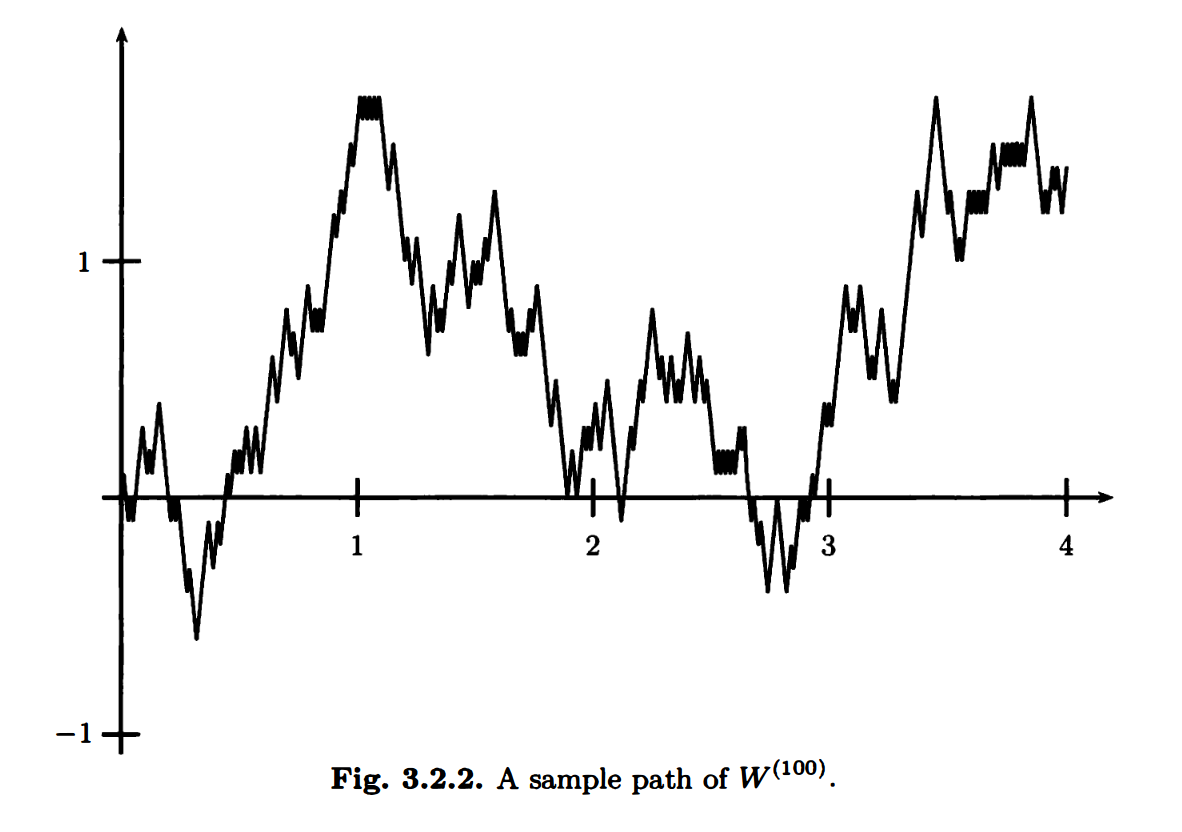
\includegraphics[width=\textwidth]{images/image.png}
    \end{column}
    \begin{column}{0.48\textwidth}
      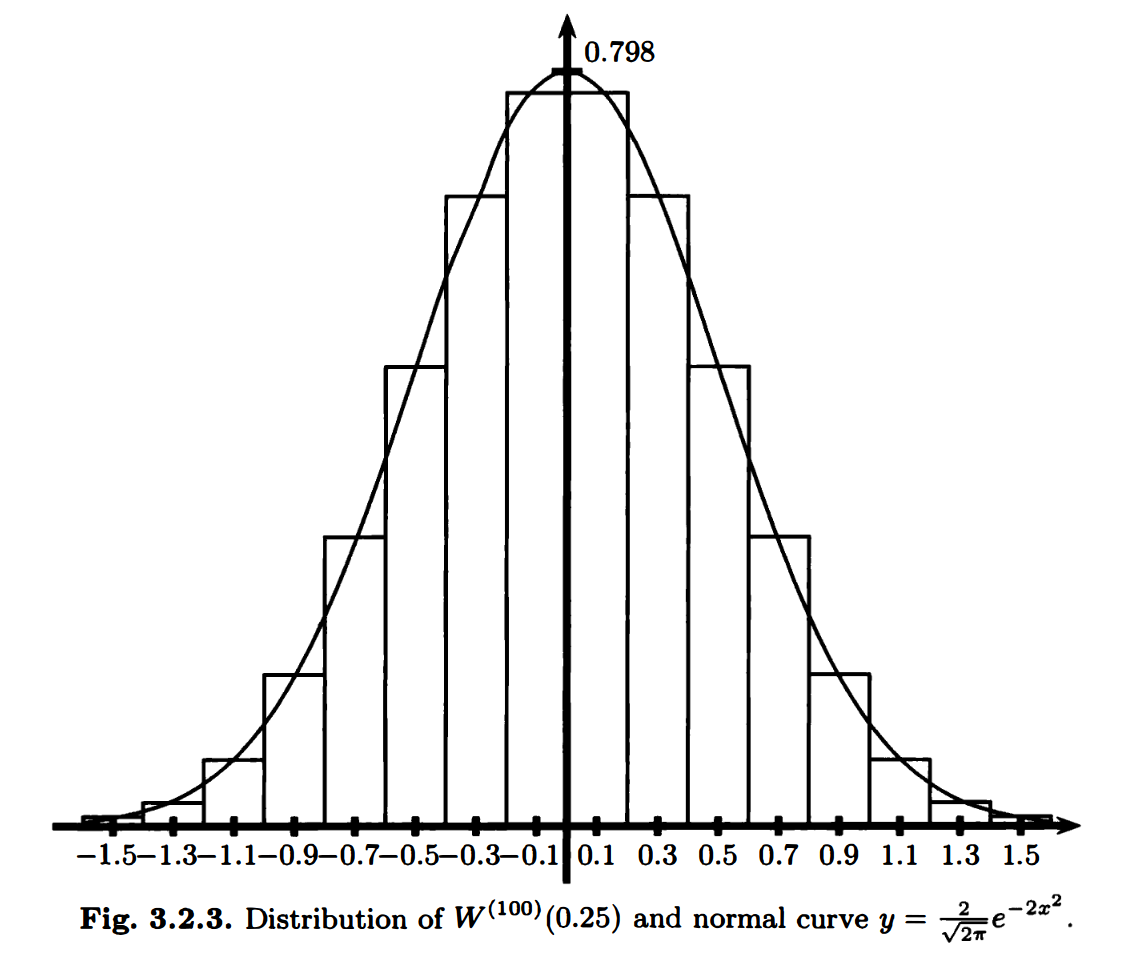
\includegraphics[width=\textwidth]{images/image2.png}
    \end{column}
  \end{columns}}
\alert<2>{\uncover<2->{As we make the increments and time steps smaller, the path becomes increasingly jagged, with increments approaching a normal distribution.}}
\end{frame}

\begin{frame}{Obtaining the Brownian Motion}
\uncover<1->{\alert<1>{We then take the limiting object of these scaled random walks (proven rigorously by taking the limit as $n \to \infty$ and using CLT.)}}

\uncover<2->{\alert<2>{By doing so, we obtain Brownian Motion.}}

\uncover<3->{
  \centering
  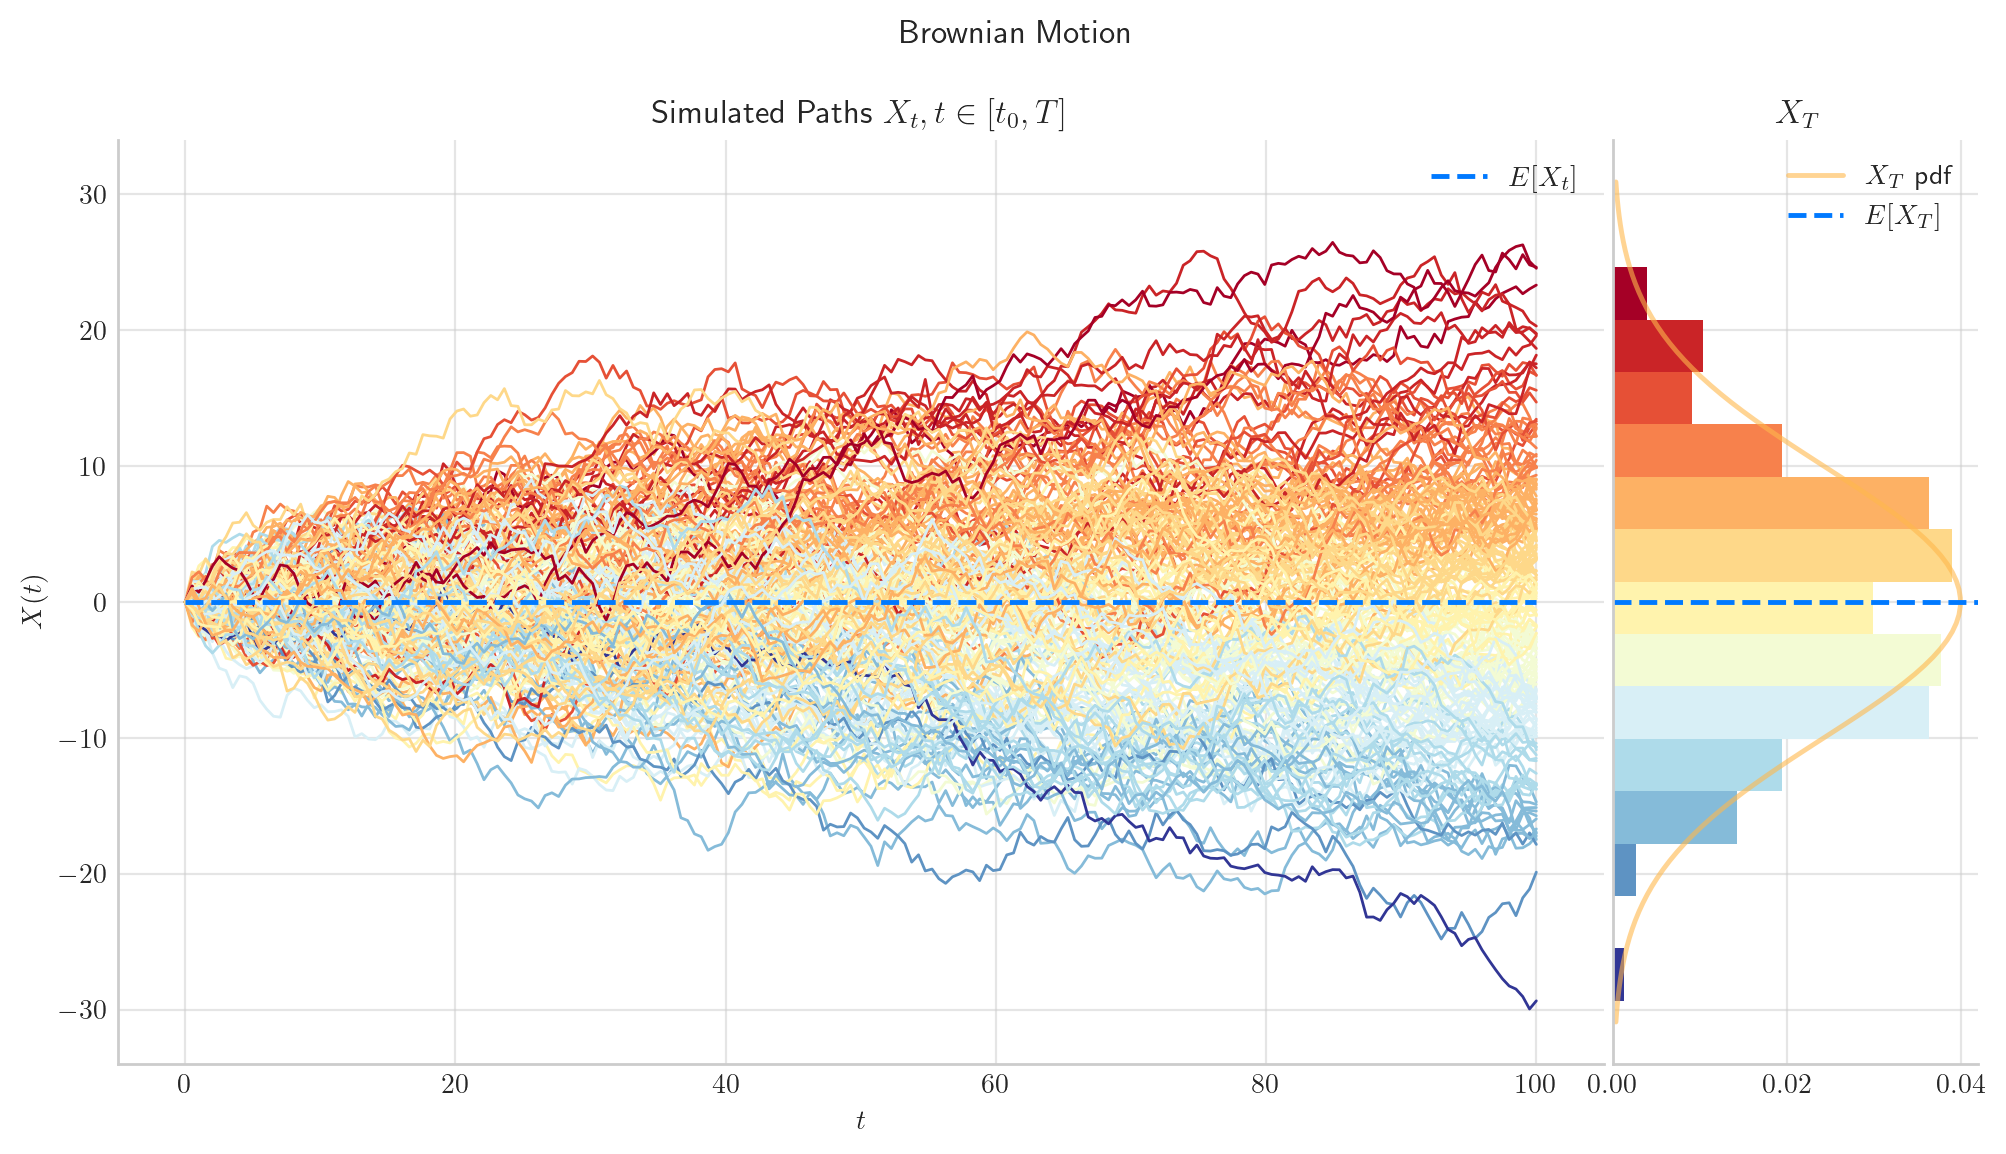
\includegraphics[width=0.7\textwidth]{images/image3.png}\\[-1em]
  \scalebox{0.75}{{\tiny Source: quantgirluk.github.io/Understanding-Quantitative-Finance}}
}
\end{frame}

\begin{frame}{Brownian Motion Properties}
\begin{definition}
Formally, a continuous function $W(t)$ dependent on $\omega \in \Omega$ is a Brownian Motion if, for all $0 = t_0 < \dots < t_m$, the increments
\[
   W(t_1) = W(t_1) - W(t_0), \dots, W(t_m) - W(t_{m-1}) 
\]
are independent and normally distributed. In addition,
\[
   E[W(t_{i+1})-W(t_i)] = 0,
\]
\[
   Var[W(t_{i+1}) - W(t_i)] = t_{i+1} - t_i.
\]
\end{definition}
\end{frame}

% What level of detail should be added here? mention risk neutral measure? discounted bond price?
\begin{frame}{The Heath-Jarrow-Morton Model}
\alert<1>{\uncover<1->{Now, we can come back to the HJM Model. 
\[
    df(t, T) = \alpha (t, T) \!\ dt + \sigma (t, T) \!\ dW(t),
\]}}
\alert<2>{\uncover<2->{Under this model, the forward rate is driven by a Brownian Motion, with rates being determined by a drift term $\alpha$ and a volatility term $\sigma$.}}

\alert<3>{\uncover<3->{Although expressing the solution to $f$ is possible in terms of an ordinary Lebesgue integral and an Ito Integral (for the Brownian Motion), in practice, numerical methods are often needed for evaluation.}}

\end{frame}

% What are the practical inputs that are fed in and what are the outputs (go into as much detail as desired about the internal processes)

% write out the f(t_j, tau_j), etc...; technically, we dont know alpha, but we use a technique called change of measure to get a "risk-neutral measure", such that any Brownian motions with drift are now a Brownian motion wrt to the new measure
\begin{frame}{Practical Implementation}
\alert<1>{\uncover<1->{The model takes in historical observations as inputs.}}

\alert<2>{\uncover<2->{Specifically, we need observations of the forward rate for various different times in the past for various different relative maturities. In addition, we also require incremental observations for some time offset $\delta$.}}

\alert<3>{\uncover<3->{Technically, this only gives us enough information to estimate $\sigma$, but through a technique called change of measure, we do not require $\alpha$.}}
\end{frame}

\begin{frame}{A Coded Example}
Below is a coded implementation of the HJM model on a dummy initial forward rate curve
\[
    f(0, T) = 0.05e^{-0.3T}.
\]

\centering
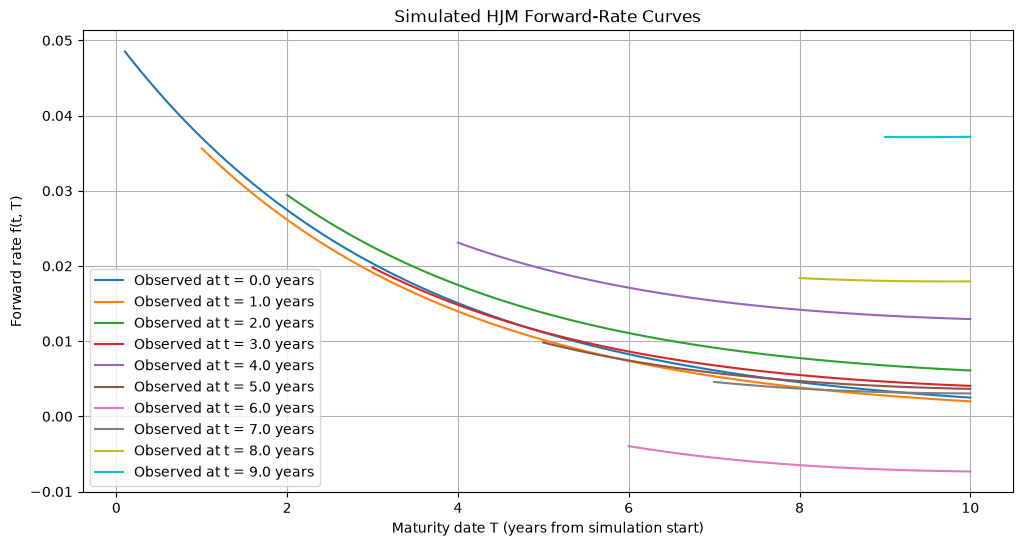
\includegraphics[width=0.9\textwidth]{images/plot.png}
\end{frame}

\begin{frame}{References}
\footnotesize

\begin{thebibliography}{9}

\bibitem{shreve2004}
Steven E. Shreve.
\newblock \emph{Stochastic Calculus for Finance II:
Continuous-Time Models}.
\newblock Springer Finance, Springer, 2004.

\end{thebibliography}

\end{frame}


\end{document}